This module of the Risk Modeller's Toolkit allows the generation of a large number of capacity curves, based on a single median curve, and information regarding the expected dispersion at each point of the curve. \\

As an example, in a study carried out by \cite{SilvaEtAl2014b}, several capacity curves were derived for 100 reinforced concrete frames with 4 storeys without seismic provisions, as illustrated in Figure \ref{fig:set_cc}. In addition to the mean and median capacity curves, an additional capacity curve was also derived using the mean geometrical and material properties of the building class of interest. From this distribution of curves, it is possible to assess the probabilistic distribution of a number of specific points, such as the yielding or ultimate capacities. Then, once adequate statistical models have been defined for these specific points, it is possible to reproduce the the distribution of capacity curves using a Monte Carlo approach. If one assumes that such distribution could be applicable to other building classes, then it is possible to produce sets of capacity curves (as a way to propagate the building-to-building variability), based on this dispersion and a capacity curve believed to be representative of the median capacity of the building class.

\begin{figure}[htb]
  \centering
      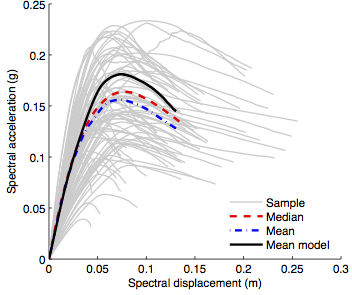
\includegraphics[width=7cm]{figures/set_capacity_curves.png}
  \caption{Capacity curves using a displacement-based adaptive pushover approach \citep{SilvaEtAl2014b}.}
  \label{fig:set_cc}
\end{figure}

To use this methodology, it is necessary to import the module \verb=point_dispersion=. Then, the spectral acceleration and displacement of the median capacity curve should be defined in the vectors \verb=Sa= and \verb=Sd=, respectively. For each point in these vectors, it is necessary to provide the corresponding variability (as a form of a coefficient of variation), in the variables \verb=Sa_cov= and \verb=Sd_cov=. The type of probabilistic distribution that should be used must be defined using the parameter \verb=type_of_dist=. Currently this module allows \verb=normal= and \verb=lognormal=. An example of the definition of these variables is provided below. In this case, the capacity curves are being defined using three points (the yielding capacity, the point of maximum force and the ultimate displacement).

\begin{Verbatim}[frame=single, commandchars=\\\{\}, samepage=true]
Sa = [0.25, 0.45, 0.35]
Sa_cov = [0.25, 0.30, 0.30]
Sd =  [0.10, 0.20, 0.50]
Sd_cov = [0.20, 0.30, 0.45]
type_dist = 'normal'
\end{Verbatim}

Within this methodology, it is also possible to specify the correlation in the spectral acceleration (\verb=Sa_corr=) and spectral displacement (\verb=Sd_corr=). If these correlation factors are set to zero, then the sampling process is carried out independently. On the other hand, if these parameters are set to one, then a full correlation is assumed, which means, for example, if a higher displacement is sampled for the yielding point, then a large displacement will also be sampled for the remaining points. Values between zero and one will lead to intermediate situations. It is also possible to control the correlation between the spectral acceleration and displacement, using the variable \verb=SaSd_corr=.
The dispersion of the synthetic capacity curves can also be controlled through the allowed number of standard deviations above or below the median capacity curve. This aspect is controlled by the parameter \verb=truncation=, which should be equal to the maximum number of allowed standard deviations. for example, a value equal to 1 signifies that all of the generated capacity curves will be within one standard deviation of the median capacity curve. Finally, the number of capacity curves that will be generated needs to be specified using the variable \verb=no_cc=. Figure \ref{fig:dispersion_cc} illustrates 100 capacity curves generated using the data provided above.

\begin{figure}[htb]
  \centering
      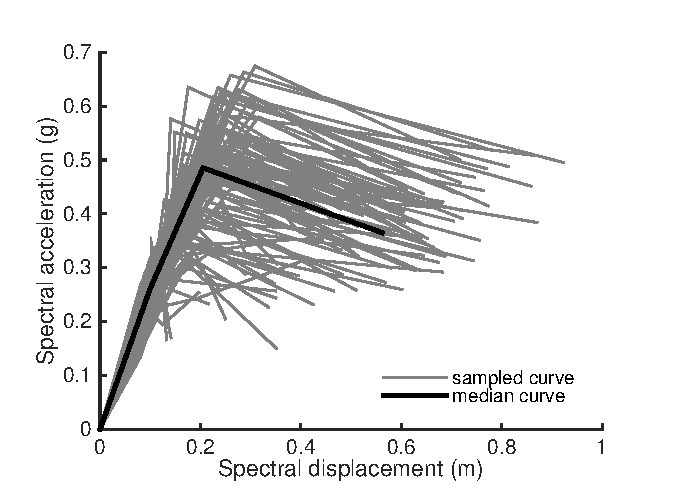
\includegraphics[width=8cm]{figures/dispersion_cc.eps}
  \caption{Capacity curves generated using the point dispersion approach.}
  \label{fig:dispersion_cc}
\end{figure}